\documentclass[11pt,letterpaper]{article}
\usepackage[T1]{fontenc}
\usepackage{lmodern}
\usepackage{graphicx}
\graphicspath{{./}{../}}
\providecommand{\pandocbounded}[1]{#1}
\usepackage{amsmath,amssymb,mathtools}
\usepackage[margin=1in,top=.85in,bottom=.85in]{geometry}
\usepackage{microtype}
\usepackage{enumitem}
\usepackage{titlesec}
\usepackage{needspace}
\usepackage[hidelinks]{hyperref}
\setlength{\parindent}{0pt}
\setlength{\parskip}{4.5pt plus 1pt minus 1pt}
\setlist{nosep,leftmargin=1.6em,topsep=4pt}
\setlength{\emergencystretch}{1.5em}
\allowdisplaybreaks[1]
\raggedbottom
\widowpenalty=10000
\clubpenalty=10000
\titleformat{\section}{\Large\bfseries}{}{0pt}{}
\titleformat{\subsubsection}{\normalsize\bfseries}{}{0pt}{}
\titleformat{\subsection}{\large\bfseries}{}{0pt}{}
\titlespacing*{\section}{0pt}{14pt}{8pt}
\titlespacing*{\subsubsection}{0pt}{9pt}{4pt}
\titlespacing*{\subsection}{0pt}{12pt}{6pt}
\newcommand{\tightlist}{\setlength{\itemsep}{0pt}\setlength{\parskip}{0pt}}
\hypersetup{pdftitle={Honours Linear Algebra - Week
3},pdfsubject={Honours Linear Algebra: 21 and 23 September 2026}}
\begin{document}
\begin{center}
{\LARGE Honours Linear Algebra - Week 3\par}
\vspace{5pt}
{\large 21 and 23 September 2026\par}
\end{center}
\vspace{4pt}
\Needspace{7\baselineskip}
\subsection{21 Sept.~/ Dimension of a
sum}\label{sept.-dimension-of-a-sum}

\textbf{Thm.1.31.} For finite-dimensional subspaces \(U,W\), \[
\dim(U+W)=\dim U+\dim W-\dim(U\cap W).
\] Proof: take a basis \(B\) of \(U\cap W\); extend to \((B,C)\) for
\(U\), \((B,D)\) for \(W\). Then \((B,C,D)\) spans \(U+W\). \[
\sum a_ib_i+\sum c_ju_j+\sum d_kw_k=0
\Rightarrow\sum d_kw_k\in U\cap W
\Rightarrow d_k=0\Rightarrow c_j=a_i=0.
\] Thus \((B,C,D)\) is a basis; count vectors. If \(U\cap W=\{0\}\),
dimensions add.

\textbf{Ex.1.52.} Distinct planes through \(0\) in \(\mathbb R^3\): \[
U+W=\mathbb R^3,\qquad \dim(U\cap W)=2+2-3=1.
\] In \(\mathbb R^4\), two planes can have zero intersection:
\(\operatorname{Span}(e_1,e_2)\) and \(\operatorname{Span}(e_3,e_4)\).

\textbf{Def.1.34--35 / several summands.} \[
V=\bigoplus_{i=1}^rU_i
\iff V=\sum_iU_i,\qquad
\left[\sum_i u_i=0,\ u_i\in U_i\Rightarrow u_i=0\ \forall i\right].
\] Equivalently \(U_j\cap\sum_{i\ne j}U_i=\{0\}\) for every \(j\); each
\(v\) has a unique decomposition \(v=\sum_i u_i\).

Pairwise zero intersections are insufficient: the \(x\)-axis, \(y\)-axis
and \(y=x\) in \(\mathbb R^2\) satisfy \[
U_i\cap U_j=\{0\}\ (i\ne j),\qquad e_1+e_2-(e_1+e_2)=0.
\]

\Needspace{7\baselineskip}
\subsection{Linear maps}\label{linear-maps}

\textbf{Def.2.1--2.} \(T:V\to W\) over the same field \(K\) is linear
iff \[
T(au+bv)=aT(u)+bT(v)\quad(a,b\in K).
\] In particular \(T(0)=0\). Notation:
\(\mathcal L(V,W)=\operatorname{Hom}(V,W)\);
\(\operatorname{End}(V)=\mathcal L(V,V)\). \[
(S+T)(v)=S(v)+T(v),\qquad(cT)(v)=cT(v).
\] \(\mathcal L(V,W)\) is a vector space. Composition is linear;
\(\operatorname{End}(V)\) is a ring under composition.

\newpage

\Needspace{7\baselineskip}
\subsection{Basis images; kernel and
image}\label{basis-images-kernel-and-image}

\textbf{Prop.2.3--4.} A linear map is determined by its values on a
basis: \[
v=\sum_j c_jb_j\quad\Rightarrow\quad T(v)=\sum_j c_jT(b_j).
\] Any chosen images of the \(b_j\) define a unique linear map. For
standard bases, \[
T:K^n\to K^m,\qquad
A=\bigl(T(e_1)\ \cdots\ T(e_n)\bigr)\in M_{m\times n}(K),\quad T(x)=Ax.
\] Images go in the \textbf{columns}.

\Needspace{4\baselineskip}
\textbf{Examples.} Zero, identity, inclusion \(U\hookrightarrow V\),
restriction \(T|_U\); also \[
\begin{aligned}
\operatorname{ev}_{t_0}:K_n[t]&\to K,&p&\mapsto p(t_0),\\
\operatorname{Tr}:M_n(K)&\to K,&A&\mapsto\sum_i a_{ii},\\
D:C^\infty(\mathbb R)&\to C^\infty(\mathbb R),&f&\mapsto f'.
\end{aligned}
\] Fourier coefficients are linear too:
\(\widehat{af+bg}(k)=a\hat f(k)+b\hat g(k)\).

\textbf{Def.2.5--6.} \[
\ker T=\{v:T(v)=0\}\le V,\qquad
\operatorname{Im}T=T(V)=\{T(v):v\in V\}\le W.
\] Closure follows from linearity. For \(D\) above,
\(\ker D=\{\text{constant functions}\}\).

\Needspace{7\baselineskip}
\subsection{23 Sept.~/ Injective,
surjective}\label{sept.-injective-surjective}

\textbf{Def.2.8--10.} \[
\begin{aligned}
T\text{ injective}&\iff T(u)=T(v)\Rightarrow u=v\iff\ker T=\{0\},\\
T\text{ surjective}&\iff\operatorname{Im}T=W,\\
T\text{ isomorphism}&\iff T\text{ injective and surjective}.
\end{aligned}
\] Kernel test: \(T(u)=T(v)\Rightarrow u-v\in\ker T\).

Injective \(\iff\) preserves every independent list. Key step: \[
\sum_i a_iT(v_i)=0\Rightarrow T\!\left(\sum_i a_iv_i\right)=0
\Rightarrow\sum_i a_iv_i=0\Rightarrow a_i=0.
\] Reverse: apply preservation to singletons \(\{v\}\), \(v\ne0\).
Surjective \(\iff\) images of a spanning set span \(W\).

\textbf{Ex.2.9--11.} Inclusion: injective. \(T:V\to T(V)\): onto. If
\(V=U\oplus W\), \[
\pi_W(u+w)=w,\qquad \ker\pi_W=U,\quad\operatorname{Im}\pi_W=W.
\]

\newpage

\Needspace{7\baselineskip}
\subsection{Isomorphisms; matrix
representation}\label{isomorphisms-matrix-representation}

\textbf{Prop.2.11--13.} An isomorphism has a unique linear inverse: \[
T^{-1}T=I_V,\qquad TT^{-1}=I_W,\qquad
(S\circ T)^{-1}=T^{-1}\circ S^{-1}.
\] Linearity: write \(w_i=T(v_i)\), then
\(T^{-1}(aw_1+bw_2)=av_1+bv_2\). For a basis
\(\mathcal B=(b_1,\ldots,b_n)\), \[
\psi_{\mathcal B}:V\xrightarrow{\sim}K^n,\quad v\mapsto[v]_{\mathcal B},
\qquad\psi_{\mathcal B}^{-1}(c)=\sum_i c_ib_i.
\] Thus finite-dimensional \(V\cong W\iff\dim_KV=\dim_KW\).

\textbf{Ex.2.12--16.} \[
K_n[t]\cong K^{n+1},\quad M_{m\times n}(K)\cong K^{mn},\quad
\mathbb C\cong\mathbb R^2\text{ over }\mathbb R\ (a+bi\mapsto(a,b)).
\] The \(xy\)-plane in \(\mathbb R^3\) is isomorphic to \(\mathbb R^2\),
though not equal to it.
\(U\times W=(U\times\{0\})\oplus(\{0\}\times W)\).

\textbf{Def.2.14.} Let \(\mathcal B\) be a basis of \(V\),
\(\mathcal C\) a basis of \(W\). Following the slides, source basis
upstairs: \[
M=[T]^{\mathcal B}_{\mathcal C}
=\bigl([T(b_1)]_{\mathcal C}\ \cdots\ [T(b_n)]_{\mathcal C}\bigr),
\qquad [T(v)]_{\mathcal C}=M[v]_{\mathcal B}.
\] \(M=\psi_{\mathcal C}\circ T\circ\psi_{\mathcal B}^{-1}\): change to
coordinates, apply \(M\), change back.

\textbf{Prop.2.18--19.} For \(U\xrightarrow{S}V\xrightarrow{T}W\), \[
[T\circ S]^{\mathcal B}_{\mathcal D}
=[T]^{\mathcal C}_{\mathcal D}[S]^{\mathcal B}_{\mathcal C}.
\] Rightmost acts first. Standard bases: \(AB\) represents \(T\circ S\);
its \(j\)-th column is \(T(S(e_j))=A b_j\).

\begin{center}
\begin{minipage}{\linewidth}
\centering
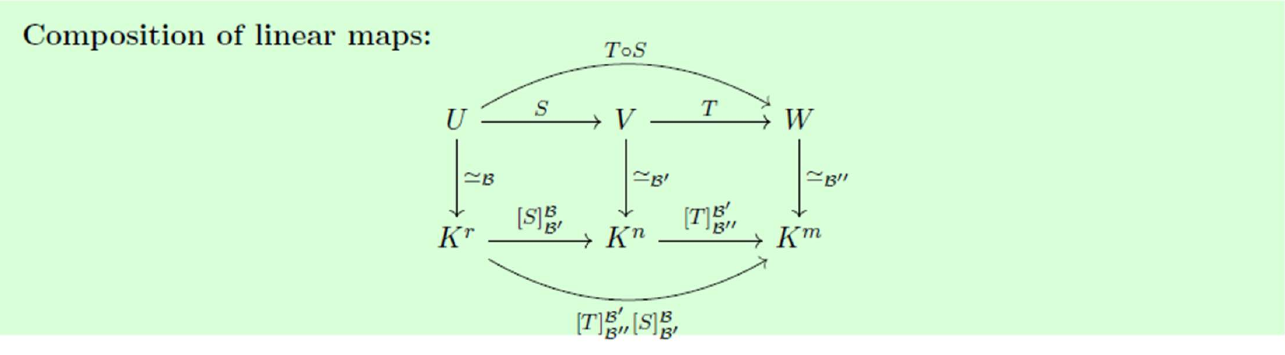
\includegraphics[width=0.86\linewidth,height=\textheight,keepaspectratio]{images/w3-composition.png}\par
{\small \emph{23 Sept., p.12.}\par}
\end{minipage}
\end{center}

\textbf{Prop.2.16 / trace.} Square \(A,B\); invertible \(Q\): \[
\operatorname{Tr}(AB)=\sum_{i,j}a_{ij}b_{ji}=\operatorname{Tr}(BA),\qquad
\operatorname{Tr}(Q^{-1}AQ)=\operatorname{Tr}(A).
\]

\newpage

\Needspace{7\baselineskip}
\subsection{Row operations; one worked
matrix}\label{row-operations-one-worked-matrix}

For \(T(x)=Ax\), \(\ker T=\operatorname{Nul}(A)\),
\(\operatorname{Im}T=\operatorname{Col}(A)\).

\textbf{Prop.2.22--24.} Row operations \(R=EA\), \(E\) invertible: \[
Rx=0\iff Ax=0,\qquad
\sum_j c_ja_j=0\iff\sum_j c_jr_j=0.
\] Same null space and same coefficients in column relations. Column
operations \(AQ\) with \(Q\) invertible preserve the column space.

\textbf{Ex.2.17--19.} \[
A=\begin{pmatrix}2&4&0&2\\1&2&3&4\\2&4&8&10\end{pmatrix}
\sim\begin{pmatrix}1&2&3&4\\0&0&1&1\\0&0&0&0\end{pmatrix}
\sim\underbrace{\begin{pmatrix}1&2&0&1\\0&0&1&1\\0&0&0&0\end{pmatrix}}_R.
\] \(Ax=0\): \(x_1+2x_2+x_4=0\), \(x_3+x_4=0\). Hence \[
x=s\begin{pmatrix}-2\\1\\0\\0\end{pmatrix}
+t\begin{pmatrix}-1\\0\\-1\\1\end{pmatrix}.
\] These two vectors form a null basis. Pivots in columns \(1,3\): \[
\operatorname{Col}(A)=\operatorname{Span}\left\{
\begin{pmatrix}2\\1\\2\end{pmatrix},
\begin{pmatrix}0\\3\\8\end{pmatrix}\right\}.
\] Use columns of \(A\), not \(R\). Here \(a_2=2a_1\), \(a_4=a_1+a_3\);
the same relations hold among columns of \(R\).

\textbf{Cor.2.25 / unique RREF.} Pivot columns occur exactly where \[
a_j\notin\operatorname{Span}(a_1,\ldots,a_{j-1}).
\] So their positions are fixed by \(A\). In RREF they are standard unit
vectors; all other columns are determined by their unchanged dependence
coefficients. Hence two RREFs coincide.

\textbf{Thm.2.29 / row rank = column rank.} \[
\dim\operatorname{Row}(A)
=\#\{\text{nonzero echelon rows}\}
=\#\{\text{pivots}\}
=\dim\operatorname{Col}(A).
\] For this \(A\): rank \(2\), nullity \(2\);
\(T:\mathbb R^4\to\mathbb R^3\) is neither injective nor onto.

\newpage

\Needspace{7\baselineskip}
\subsection{Rank--nullity}\label{ranknullity}

\textbf{Def.2.28.} \(\operatorname{rank}T=\dim\operatorname{Im}T\),
\(\operatorname{nullity}T=\dim\ker T\).

\textbf{Thm.2.30.} \(\dim V<\infty\), \(T:V\to W\) linear: \[
\boxed{\dim V=\dim\ker T+\dim\operatorname{Im}T.}
\] Proof / lift a basis of the image. Let \((w_1,\ldots,w_r)\) be a
basis of \(\operatorname{Im}T\); choose \(u_i\) with \(T(u_i)=w_i\), and
set \(H=\operatorname{Span}(u_1,\ldots,u_r)\). \[
\sum_i c_iu_i=0\Rightarrow\sum_i c_iw_i=0\Rightarrow c_i=0,
\qquad \dim H=r.
\] Likewise \(h\in H\cap\ker T\Rightarrow h=\sum c_iu_i\),
\(\sum c_iw_i=0\Rightarrow h=0\). For any \(v\in V\), write
\(T(v)=\sum b_iw_i\). Then \[
v=\underbrace{\left(v-\sum_i b_iu_i\right)}_{\in\ker T}
+\underbrace{\sum_i b_iu_i}_{\in H}.
\] Thus \(V=\ker T\oplus H\),
\(T|_H:H\xrightarrow{\sim}\operatorname{Im}T\); count dimensions.

\textbf{Consequences.} \(A\in M_{m\times n}(K)\), rank \(r\): \[
\begin{aligned}
\operatorname{nullity}A&=n-r,\\
T\text{ injective}&\iff r=n\quad(\text{all columns pivot}),\\
T\text{ surjective}&\iff r=m\quad(\text{every row has a pivot}).
\end{aligned}
\] If \(\dim V=\dim W<\infty\): injective \(\iff\) surjective \(\iff\)
isomorphism. For injective \(T\), every subspace \(U\) satisfies
\(\dim T(U)=\dim U\) (its basis maps to a basis). Conversely, this
equality for all \(U\) forces injectivity: use
\(U=\operatorname{Span}(v)\) for \(v\ne0\).

\textbf{Ex. / finite-dimensional condition.} On \(\mathbb R[t]\), \[
D(p)=p'\text{ is onto but not injective},\qquad
M(p)=tp\text{ is injective but not onto}.
\] For \(Ax=b\): no solution if \(b\notin\operatorname{Col}(A)\);
otherwise \[
\{x:Ax=b\}=x_p+\operatorname{Nul}(A),\qquad n-r\text{ free parameters}.
\]
\end{document}
